\subsection{Impresión 3D}

\par
Es necesario definir el concepto de prototipo porque es el punto de partida para el desarrollo de la tecnología de Prototipado Rapido y consecuentemente, para las impresoras tridimensionales. Podemos definir como prototipo al primer ejemplar que se fabrica de una figura, un invento o elemento físico, y sirve de modelo para fabricar otros iguales.  

\par \noindent
Los prototipos tiene el propósito de probar suposiciones formuladas en busca de una solución a un problema determinado. Ademas se convierten en un diseño enfocado al usuario, donde es necesario un proceso interactivo entre el propio diseñador y el consumidor. Así mismo, todos los prototipos son objetos de desarrollo de bajo costo, pero en muchas ocasiones la necesidad de elaborar varios prototipos o de realizar un prototipo con una estética cuidada, eleva los costes de producción. Por lo tanto, el alto coste de producción de prototipos y tiempo de ejecución de los mismos puede suponer un problema.

\par \noindent
Los sistemas de Prototipado Rápido surgen con la necesidad de solventar estos problemas en el uso de prototipos, se busca por lo tanto, una manera de elaborarlos con un aspecto cuidado y atractivo para el usuario, con un método de fabricación rápido y fácil de modificar, económicos y que pueden ser probados por el consumidor. Por consiguiente, esta herramienta resultará útil y funcional. Rápidamente estos sistemas de construcción aditiva partirán del desarrollo tecnológico de maquinara destinada a uso industrial\cite{impresoras3d-valverde}. 

\begin{figure}[H]
	\centering
	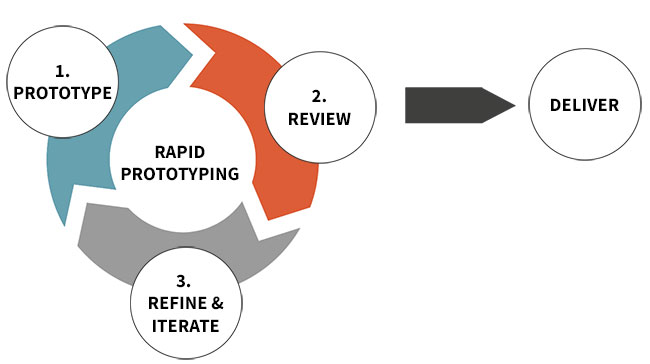
\includegraphics[width=0.5\textwidth]{impresion1.jpg}
	\caption{Ciclo del Prototipado Rapido}
\end{figure}

\par \noindent
El Prototipado Rápido se convierte así, en un proceso utilizado para la fabricación de prototipos, los cuales, como hemos visto, son objetos que no estan diseñados a uso final, sino más bien a modo de prueba de diseño\cite{impresoras3d-valverde}.

\par \noindent
La impresión 3D, también conocida como impresión tridimensional, es un método para
producir objetos tridimensionales con un aparato tecnológico al colocar varias capas
bidimensionales de cierto material una sobre la otra. El proceso es similar a la impresión
bidimensional en la cual se coloca tinta sobre papel, sin embargo, en la impresión
tridimensional se coloca plástico sobre una superficie que nos permite fabricar objetos de tres
dimensiones. Esta tecnología se utiliza principalmente en la producción de prototipos durante
el diseño de algún nuevo producto.

\par \noindent
Durante los últimos años, la tecnología de impresión tridimensional ha avanzado de
manera exponencial. Este tipo de impresoras se han vuelto cada vez más accesibles y por ello
ahora es común encontrarlas en fábricas, industrias, instituciones educativas, instituciones de
investigación e inclusive para uso personal\cite{impresoras3d-monterrey}.

\subsubsection{Técnicas de Impresión 3D}

\par \noindent
Hablaremos de las principales técnicas comerciales de impresión 3D; ya que, la impresión 3D es una tecnología de hace muchos años. No fue hasta a mediados de la década del 2000 que la impresoras 3D comenzaron a bajar sus precios y apuntados a un mercado menos especializado.

\begin{figure}[H]
	\centering
	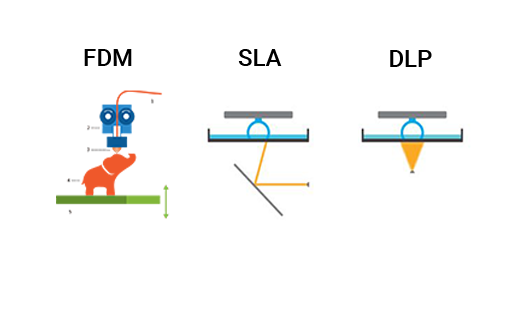
\includegraphics[width=0.8\textwidth]{impresion2.png}
	\caption{Principales Técnicas Comerciales de Impresion 3D}
\end{figure}

\paragraph{FDM (Modelado por Disposición de Hilo Fundido)}
Consiste en la deposición por capas de material normalmente construido por filamentos de polímeros termoplásticos, que se funden y se extruyen por medio de una boquilla, solidificándose cuando salen de dicha boquilla al exterior, ver figura 2.18. (FDM).\cite{impresoras3d-valverde}.

\begin{figure}[H]
	\centering
	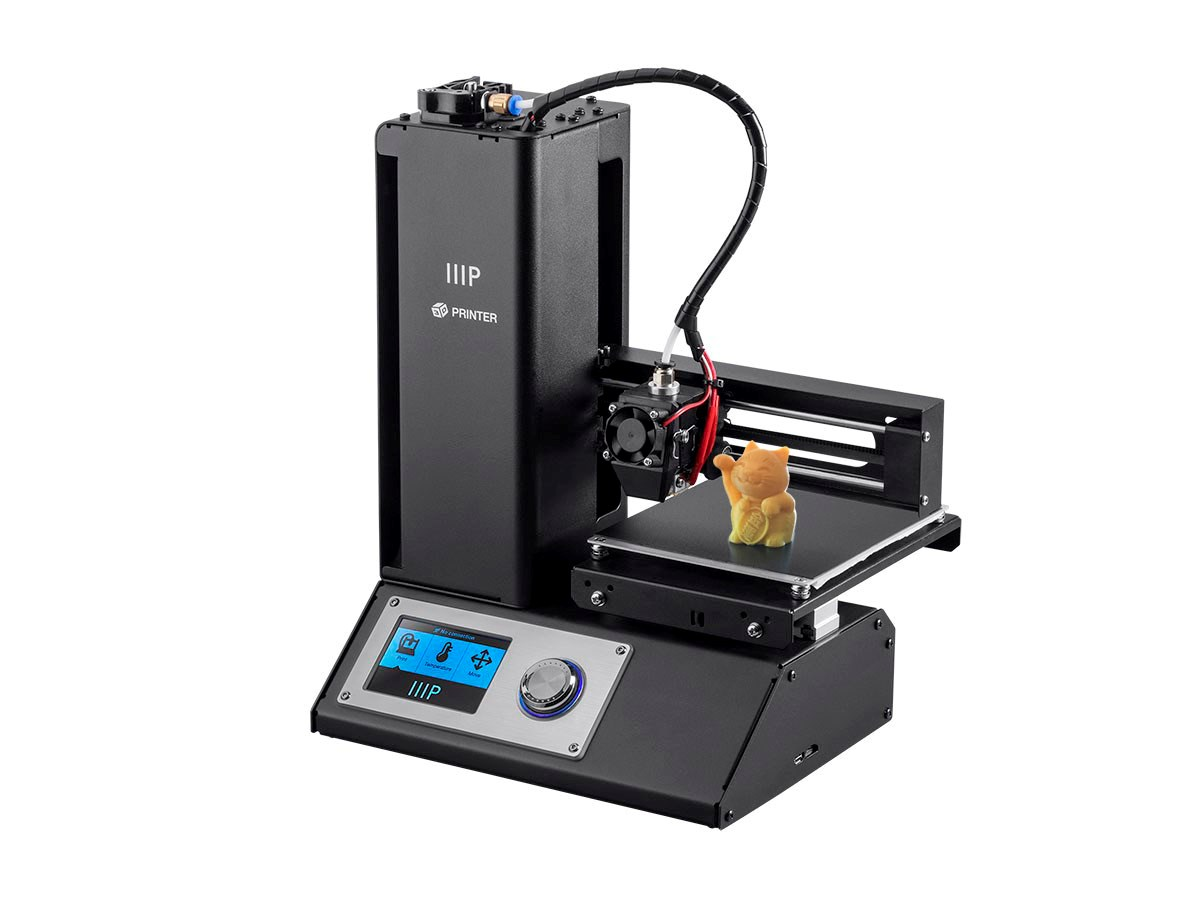
\includegraphics[width=0.5\textwidth]{impresion3.jpg}
	\caption{Impresora FDM: MP Select Mini V2 de Monoprice.}
\end{figure}

\paragraph{SLA (Estereografía)}
Se basa en las propiedades de una resina fotosensible que se solidifica mediante la proyección de un láser (UV) de frecuencia y potencia concreta, ver figura 2.18. (SLA)\cite{impresoras3d-valverde}.

\begin{figure}[H]
	\centering
	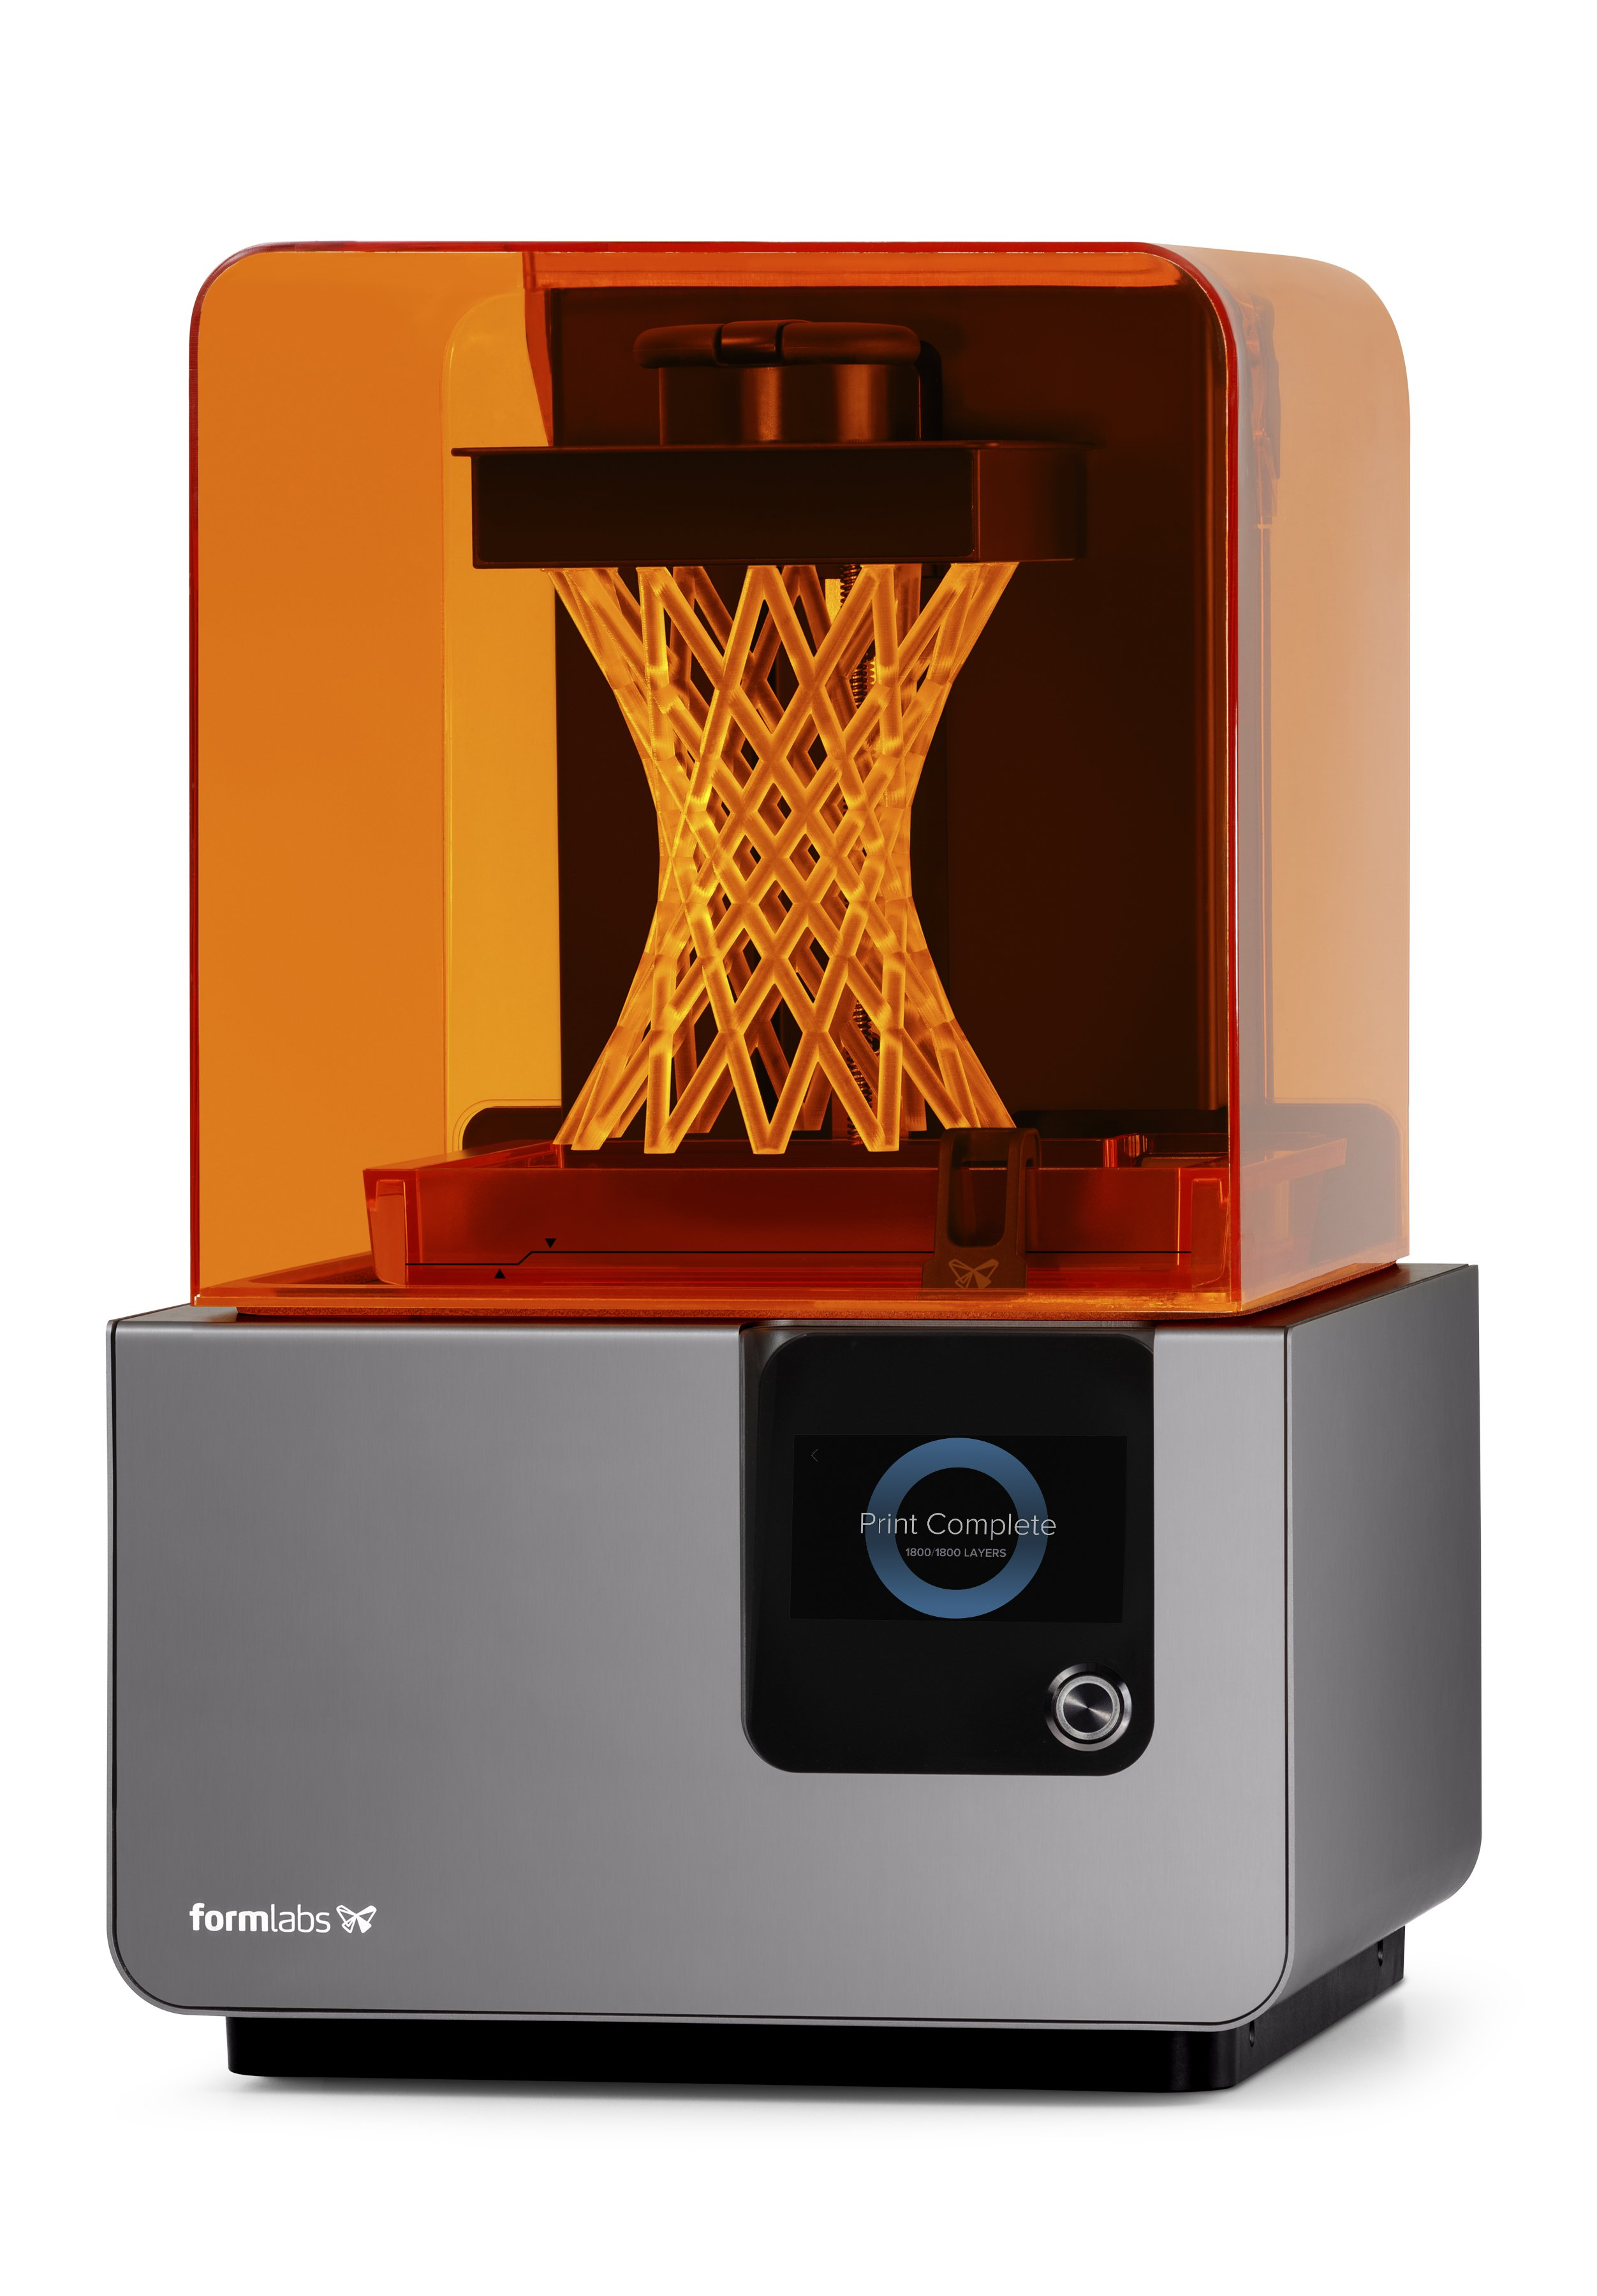
\includegraphics[width=0.3\textwidth]{impresion4.jpg}
	\caption{Impresora SLA: Form2 de Formlabs.}
\end{figure}

\paragraph{DLP (Procesamiento de Luz Digital)}
En este proceso, una cubeta de polímero líquido se expone a la luz de un proyector DLP en condiciones de seguridad. El proyector DLP muestra la imagen del modelo 3D en el polímero líquido, ver figura 2.18 (DLP). El polímero líquido expuesto se endurece y la placa de construcción se mueve hacia abajo y el polímero líquido queda una vez más expuesto a la luz. El proceso se repite hasta que el modelo 3D se completa y la tina se drena de líquido, lo que revela el modelo solidificado\cite{impresoras3d-blog}.

\begin{figure}[H]
	\centering
	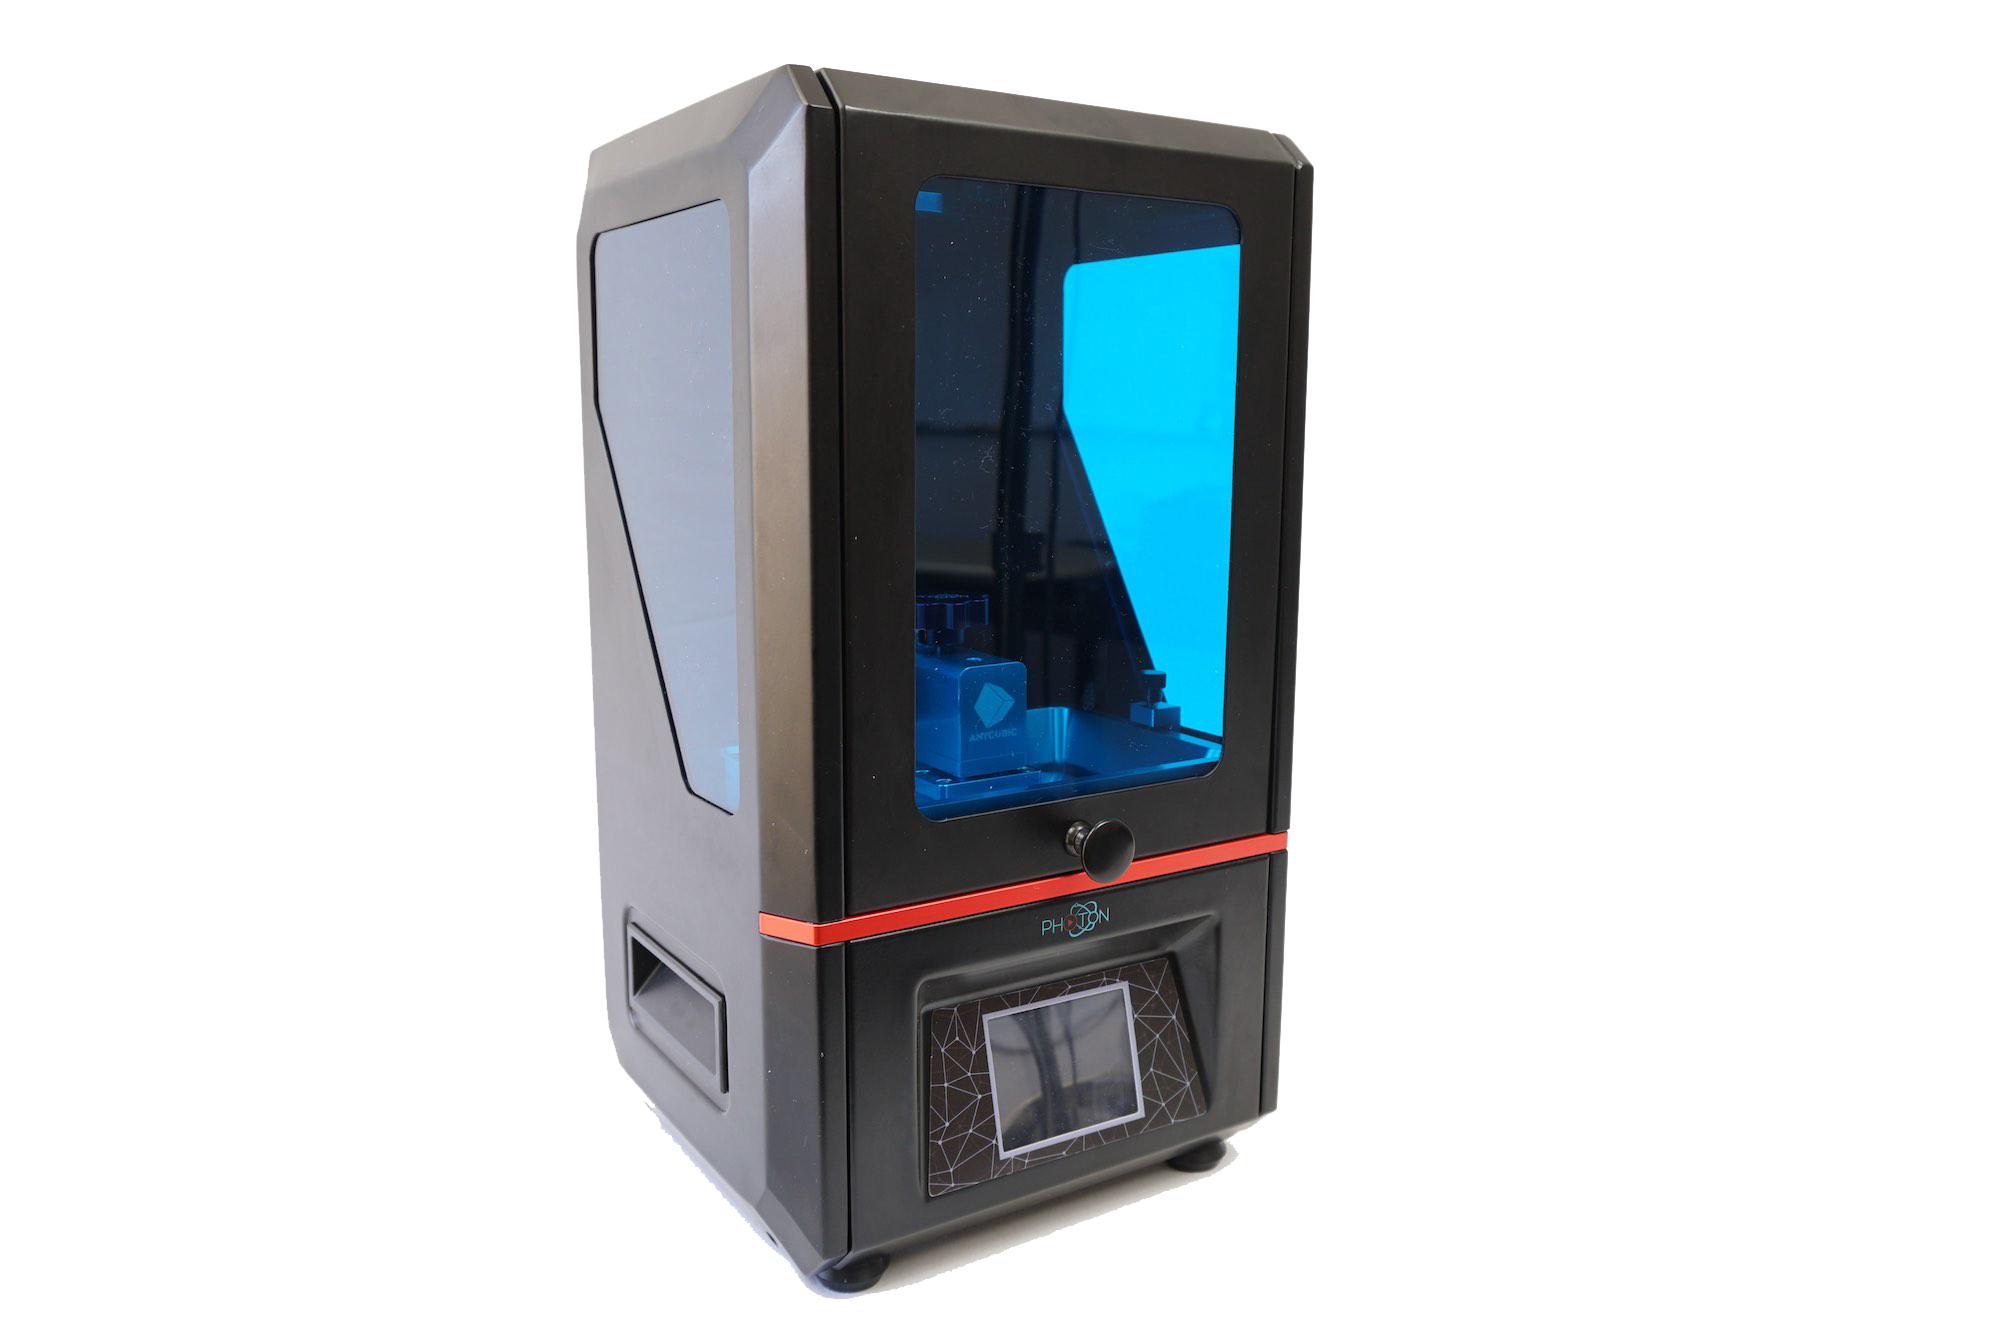
\includegraphics[width=0.5\textwidth]{impresion5.jpg}
	\caption{Impresora DLP: LCD Photon de Anycubic.}
\end{figure}

